\chapter{Klase podataka}

Razmatranjem slučajeva upotrebe zaključeno je da je za funkcionisanje informacionog sistema najbitnije čuvati sledeće podatke:
\begin{enumerate}
\item Podaci o zaposlenima
\item Podaci o slikama
\item Podaci o autorstvu
\item Podaci o izdanjima
\item Podaci o ugovorima
\item Podaci o konkursima
\end{enumerate}

\begin{figure}[htp]
    \centering
    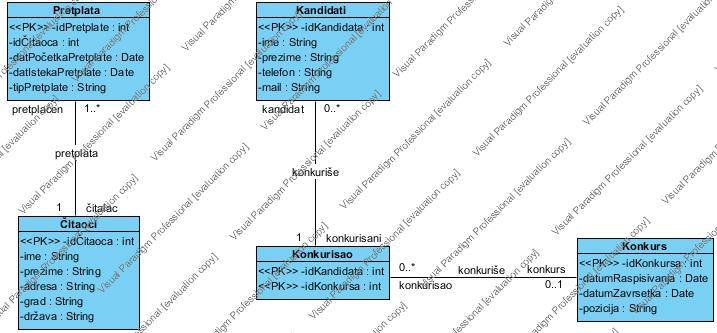
\includegraphics[width=0.9\textwidth]{slike/konkurs-pretplata}
    \caption{Klasni dijagram 1. deo}
    \label{klase1}
\end{figure}    

\begin{figure}[htp]
    \centering
    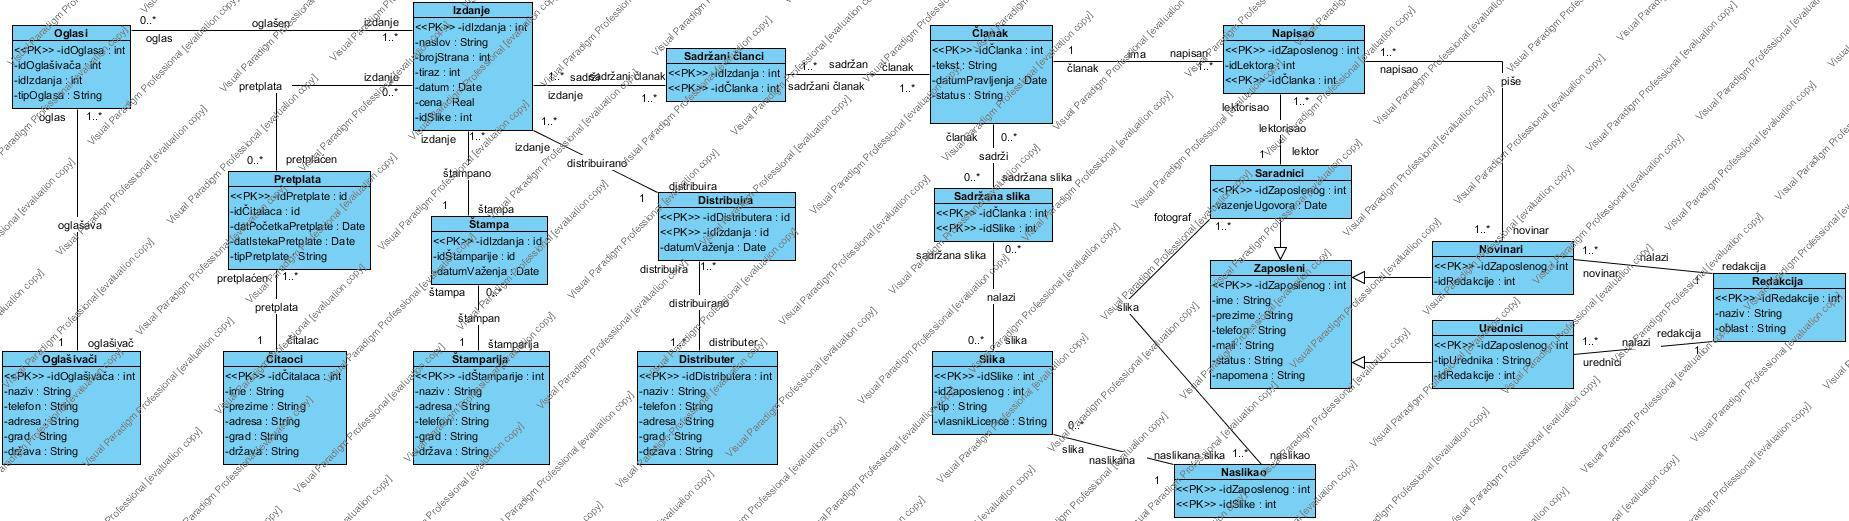
\includegraphics[width=0.9\textheight, angle=90]{slike/klasni_dijagram}
    \caption{Klasni dijagram 2. deo}
    \label{klase2}
\end{figure}    



\newpage

\section{Podaci o zaposlenima}
Klasa \textbf{zaposleni} i klase koje se izvode iz nje su ključni deo informacionog sistema. Klase koje su izvedene su \textbf{urednik}, \textbf{novinar} i \textbf{saradnik}. One preuzimaju sve atribute iz roditeljske klase i dodaju sebi specifične. \\

Kod \textbf{urednik} to je tip urednika i identifikacija redakcije kojoj urednik pripada, kod \textbf{novinar}  to je  identifikacija redakcije kojoj novinar pripada, kod \textbf{saradnik} to je podatak do kad saradnik ima važeći ugovor sa izdavaštvom. \vspace{5mm}

\noindent \textbf{Zaposleni}
\begin{enumerate}
\item Identifikacioni broj zaposlenog (PK)
\item Ime
\item Prezime
\item Telefon
\item Adresa
\item  Imejl
\item Status (može biti "stalni", "honorarni" ili "bivši")
\item Napomena (za dodatne informacije)
\end{enumerate} \vspace{5mm}

\noindent \textbf{Urednik}
\begin{enumerate}
\item Identifikacioni broj zaposlenog (PK/SK)
\item Tip urednika (može biti "glavni", "obični" ili "grafički")
\item Identifikacioni broj redakcije (SK)
\end{enumerate} \vspace{5mm}

\noindent \textbf{Novinar}
\begin{enumerate}
\item Identifikacioni broj zaposlenog (PK/SK)
\item Identifikacioni broj redakcije (SK)
\end{enumerate} \vspace{5mm}

\noindent \textbf{Saradnik}
\begin{enumerate}
\item Identifikacioni broj zaposlenog (PK/SK)
\item Važenje ugovora (mora biti Null za stalne saradnike)
\end{enumerate} \vspace{5mm}

\section{Podaci o slikama}
Klasa \textbf{slika} pamti autora slike ukoliko ju je zaposleni napravio, njen tip (fotografija, ilustracija) kao i vlasnika licence ukoliko je slika licencirana od nekuda. 

\noindent \textbf{Slika}
\begin{enumerate}
\item Identifikacioni broj slike (PK)
\item Identifikacioni broj saradnika koji je napravio sliku (SK)
\item Tip (fotografija ili ilustracija)
\item Vlasnik Licence
\end{enumerate} \vspace{5mm}


\section{Podaci o autorstvu}

Neki članak može biti biti napisan od jednog ili više novinara. Klasa \textbf{Napisao} čuva podatke o tome koji su novinari napisali članak i koji je lektor lektorisao tekst.

\noindent \textbf{Napisao}
\begin{enumerate}
\item Identifikacioni broj članka (PK/SK)
\item Identifikacioni broj novinara (PK/SK)
\item Identifikacioni broj Lektora (Saradnika)
\end{enumerate} \vspace{5mm}

\section{Podaci o izdanjima}
O izdanjima se čuvaju informacije o datumu izdavanja, tiražu, broju strana, ceni u dinarima, slici koja se koristi kao naslovna strana i spisku članaka koji se nalaze u okviru izdanja. Spisak članaka se nalazi u okviru klase \textbf{Sadržani članci} koja pored identifikacionig broja izdanja čuva i identifikacioni broj članka i broj strane na kojoj se dati članak pojavljuje 


\noindent \textbf{Izdanje}
\begin{enumerate}
\item Identifikacioni broj izdanja (PK)
\item Naslov
\item Broj strana
\item Tiraž
\item Datum izdavanja
\item Cena
\item Identifikacioni broj slike koja služi kao naslovna strana (SK)
\end{enumerate} \vspace{5mm}


\noindent \textbf{Sadržani članci}
\begin{enumerate}
\item Identifikacioni broj izdanja (PK/SK)
\item Identifikacioni broj članka (PK/SK)
\item Broj strane na kojoj se članak pojavljuje
\end{enumerate} \vspace{5mm}

\section{Podaci o ugovorima}
Podaci o ugovorima su oni podaci koji se odnose na saradnju sa spoljnim entitetima i same entitete. Tu spadaju:\\

\noindent \textbf{Distributeri}
\begin{enumerate}
\item Identifikacioni broj distributera (PK)
\item Naziv
\item Telefon
\item Adresae
\item Grad
\item Država
\item Dužina ugovora
\end{enumerate} \vspace{5mm}

\noindent \textbf{Distribuira}
\begin{enumerate}
\item Identifikacioni broj izdanja (PK/SK)
\item Identifikacioni broj distributera (PK/SK)
\end{enumerate} \vspace{5mm}

\noindent \textbf{Štamparije}
\begin{enumerate}
\item Identifikacioni broj štamparije (PK)
\item Naziv
\item Telefon
\item Adresa
\item Grad
\item Država
\item Dužina ugovora
\end{enumerate} \vspace{5mm}

\noindent \textbf{Štampa}
\begin{enumerate}
\item Identifikacioni broj izdanja (PK/SK)
\item Identifikacioni broj štamparije (SK)
\end{enumerate} \vspace{5mm}

\noindent \textbf{Čitaoci}
\begin{enumerate}
\item Identifikacioni broj čitaoca (PK)
\item Ime
\item Prezime
\item Telefon
\item Adresa
\item Grad
\item Država
\end{enumerate} \vspace{5mm}

\noindent \textbf{Pretplate}
\begin{enumerate}
\item Identifikacioni broj pretplate (PK)
\item Identifikacioni broj čitaoca (SK)
\item DatumPočetka
\item DatumKraja
\item TipPretplate (na pisano ili Internet izdanje)
\end{enumerate} \vspace{5mm}

\noindent \textbf{Oglašivači}
\begin{enumerate}
\item Identifikacioni broj oglašivača (PK)
\item Naziv
\item Telefon
\item Adresa
\item Grad
\item Država
\end{enumerate} \vspace{5mm}

\noindent \textbf{Oglasi}
\begin{enumerate}
\item Identifikacioni broj oglasa (PK)
\item Identifikacioni broj oglasa (SK)
\item Identifikacioni broj izdanja (SK)
\item TipOglasa
\item Strana
\end{enumerate}  \vspace{5mm}

\section{Podaci o konkursima}
Klasa \textbf{konkurs} čuva podatke o raspisanim konkursima za datu poziciju i od kad do kad traju. \textbf{Kandidat} čuva podatke o potencijalnim zaposlenima dok \textbf{konkurisao} vezuje te dve klase.

\noindent \textbf{Konkurs}
\begin{enumerate}
\item Identifikacioni broj konkursa (PK)
\item Datum raspisivanja
\item Datum završretka
\item Pozicija (za koju se konkuriše)
\item Napomena
\end{enumerate}  \vspace{5mm}

\noindent \textbf{Konkurisao}
\begin{enumerate}
\item Identifikacioni broj konkursa (PK/SK)
\item Identifikacioni broj kandidata (PK/SK)
\end{enumerate}  \vspace{5mm}


\noindent \textbf{Kandidat}
\begin{enumerate}
\item Identifikacioni broj kandidata (PK)
\item Ime
\item Prezime
\item Telefon
\item mail
\end{enumerate}  \vspace{5mm}

